\documentclass[brazil,a4paper,12pt]{article}

\usepackage{fullpage}
\usepackage{fancyvrb}
\usepackage[brazil]{babel}
\usepackage[utf8]{inputenc}
\usepackage{graphicx}
\usepackage{booktabs}

\begin{document}

\begin{center}
\LARGE
\textbf{Mineração de Dados}\\
\textbf{TP2: Brasil X Holanda}\\
\end{center}
\begin{center}
\textbf{Aluno: Flavio Vinicius Diniz de Figueiredo}
\end{center}

\section{Descrição}

O objetivo do TP foi de realizar as seguintes três etapas em uma base de dados 
coletada do Twitter~\footnote{\texttt{http://www.twitter.com}} durante o jogo
do Brasil contra a Holanda na copa de 2010:

\begin{description}

\item [Agrupamento de dados] Os dados da base original são compostos de tweets em 
sua maioria na língua portuguesa. Foi requisitado que o aluno agrupasse os tweets
com uma granularidade temporal de 5 minutos; ou seja, ao invés de analisar todos
os tweets como a base de dados, novas bases eram para ser geradas com granularidade
de 5 minutos cada. 

\item [Limpeza de dados] Além do agrupamento, foi requisitado que o aluno tratasse os 
dados de forma a reduzir variações textuais. A escolha de técnicas de limpeza de dados
ficou a critério do aluno.

\item [Termos Frequentes] Após a limpeza e agrupamento dos dados, foi requisitado
do aluno a mineração dos termos e/ou conjunto de termos mais frequentes em cada
base agrupada. Não foi requisitada a execução de nenhum algoritmo específico,
assim escolha da metodologia de mineração de conjuntos de termos ficou a critério
do aluno.

\end{description}

\noindent No fim de cada seção indicamos quais arquivos contém os scripts
utilizados na análise.

\section{Agrupamento de Dados}

O conjunto de dados originais era composto de 174171 tweets em um intervalo de 2h. 
O primeiro tweet foi registrado às 14:00, hora que o jogo foi iniciado, enquanto
o último foi registrado às pouco após 16:00, alguns minutos após o término do jogo. 
Como foi requisitado ao agrupamento em intervalos de 5 minutos, um total de 25
grupos foram gerados ($\frac{2h}{5mins} + 1$). O último grupo existe pois os tweets
chegam a passar às 15:59:59.

A Figura~\ref{fig:groups} mostra a quantidade de tweets em cada intervalo de 5
minutos. Na figura, podemos ver um pico em aproximadamente no intervalo
\emph{[14:10-14:15)}, possivelmente devido ao primeiro gol do Brasil. O segundo
tempo foi iniciado aproximadamente às 15:00, logo após este início o número de 
tweets cai significativamente e volta a subir no intervalo \emph{[15:10-15:15)},
devido ao primeiro gol da Holanda. O maior pico de tweets foi no intervalo
\emph{[15:30-15:35)}, neste intervalo houve o segundo gol da Holanda e a
falta de Felipe Melo. Após o término do jogo, vemos o número de tweets cair
significativamente.

\begin{figure}
\centering
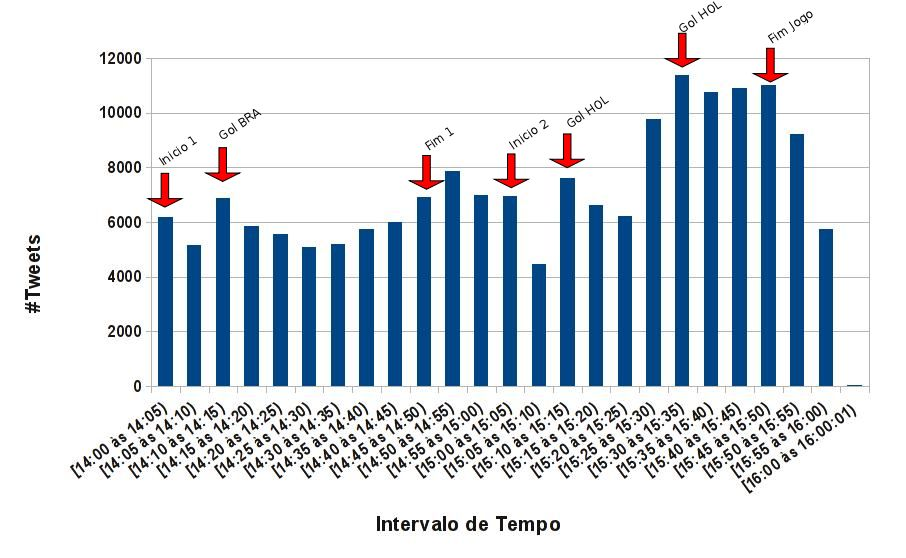
\includegraphics[scale=0.4]{group-hist.jpg}
\caption{Número de tweets em cada intervalo de tempo}
\label{fig:groups}
\end{figure}

\subsection{Código}
\begin{verbatim}
src/dm/tp2/twitter_io.py
src/dm/tp2/test/test_twitter_io.py
src/dm/tp2/scripts/parse_raw.py
\end{verbatim}

\section{Limpeza Dados}

Para limpeza de dados foram realizadas as seguintes etapas:

\begin{enumerate}
\item Inicial foram identificados os termos de cada tweet com o uso 
de um expressão regular. Com esta expressão eram 
retornados os seguintes termos: placares de jogos (p.ex. 1x1, 1x0);
termos alfanuméricos ($[a-zA-z0-9]+$); hashtags e menções a outros
usuários. Qualquer termos que não seguisse tais regras eram descartados,
assim podemos focar um subconjunto de termos legíveis.

\item Após a identificação de termos, os mesmos foram convertidos para
sua forma {\it lowercase}.

\item Dos termos restantes, filtramos as {\it stopwords} da língua
portuguesa. Como tais palavras são muito frequentes e trazem pouca
informação, é geralmente recomendado o filtro destas.

\item Por fim, palavras acentuadas foram convertidas para a forma
não acentuada (p.ex ``não'' vira ``nao''). Isto foi feito para
compensar os diversos erros de escrita que usuários cometem na 
Internet.

\end{enumerate}

\noindent Tais técnicas são padrões no tratamento de dados textuais 
tanto para mineração de dados como para recuperação de informação.
Para mais detalhes, ver o Capítulo 6.6 do livro Modern Information Retrieval~\cite{baeza2010modern}.

\subsection{Código}

\begin{verbatim}
src/dm/tp2/twitter_io.py
src/dm/tp2/test/test_twitter_io.py
src/dm/tp2/scripts/parse_raw.py
\end{verbatim}

\section{Termos Frequentes}

A última etapa do TP foi a mineração de conjunto de termos (pós filtro)
frequentes em cada intervalo de tempo. Para fins de comparação fizemos
uso de três algoritmos diferentes de termos frequentes: o 
\textsc{FPGrowth}, que minera todos os conjuntos acima do suporte mínimo;
o \textsc{Charm}, que reduz os conjuntos minerados para serem conjuntos
fechados; e, por fim, usamos um algoritmo que minera 
{\it collocations}~\footnote{\texttt{http://en.wikipedia.org/wiki/Collocation}}, 
que são sequencias frequentes de palavras (sequencias de tamanho 3 no
nosso caso). A descrição dos algoritmos \textsc{FPGrowth} e \textsc{Charm}
podem ser encontradas no livro da disciplina~\cite{meira}, neste trabalho
fizemos uso das implementações na biblioteca 
SPMF~\footnote{\texttt{http://www.philippe-fournier-viger.com/spmf/}}. A
mineração de collocations foi feita usando a biblioteca 
NLTK~\footnote{\texttt{http://www.nltk.org/}}.

\subsection{Resultados}

Como seria inviável mostrar os padrões mais frequentes para todos os intervalos
de tempo, decidimos mostrar aqui na documentação apenas os 20 conjuntos mais
frequentes no intervalo \emph{[15:30-15:35)} para o algoritmo de collocations. 
Este não só é o intervalo com mais tweets, como também foi quando ocorreu o 
segundo gol a Holanda e as faltas de Felipe Melo. Como pedido, junto com a 
documentação estamos entregando os 50 conjuntos mais frequentes ordenados por 
intervalo de tempo em arquivos separado (um para cada algoritmo). 
Tanto para o arquivo, como para o exemplo abaixo, fixamos o suporte
mínimo dos algoritmos como sendo $0.01$. Com este suporte baixo, foi garantido
mais de $50$ conjuntos para todos os algoritmos. 

Decidimos mostrar o algoritmo de collocations pois ele apresentou os resultados 
de mais fácil interpretação. Isto é devido ao fato de minerar sequências de tamanho
3. O \textsc{FPGrowth} e \textsc{Charm} minera sequências de tamanho arbitrário,
assim a mais frequentes acabam sendo termos únicos. Abaixo mostramos
os 20 conjuntos mais frequentes no intervalo \emph{[15:30-15:35)} para o algoritmo de collocations.

\begin{verbatim}
('#br', '#br', '#br') 0.00968859430889
('coloc', 'ronald', 'gauch') 0.00281645183398
('dung', 'coloc', 'ronald') 0.00281645183398
('ronald', 'gauch', 'gans') 0.00281645183398
('calm', 'gent', 'daqu') 0.0028070636612
('daqu', 'pouc', 'dung') 0.0028070636612
('gans', 'gent', 'vir') 0.0028070636612
('gauch', 'gans', 'gent') 0.0028070636612
('gent', 'daqu', 'pouc') 0.0028070636612
('pouc', 'dung', 'coloc') 0.0028070636612
('gent', 'vir', 'ai') 0.00279767548842
('vir', 'ai', '#cop') 0.0025723593417
('@kibeloco', 'calm', 'gent') 0.0025254184778
('2', '1', '#br') 0.00107025169691
('#ned', '2', '1') 0.00104208717857
('felip', 'mel', 'nao') 0.000910652759653
('http', 'bit', 'ly') 0.000901264586873
('14', 'min', '14') 0.000844935550194
('14', 'tens', 'minut') 0.000844935550194
\end{verbatim}

Dos exemplos acima podemos ver menções a jogadores que não foram para
a copa, Ronaldinho Gaúcho, um possível indicativo de que os torcedores
não estavam satisfeitos com a escalação. Vemos também menções ao segundo
gol coma hashtag $\#ned$. Além de menções negativas a Felipe Melo. Por fim,
temos tweets esperançosos indicando que ainda faltavam 14 minutos.

\subsection{Código}

\begin{verbatim}
src/dm/tp2/scripts/create_itemsets.py
src/dm/tp2/scripts/spmf/dm/main/MineSetsCharm.java
src/dm/tp2/scripts/spmf/dm/main/MineSetsFP.java
src/dm/tp2/scripts/collocations.py
src/dm/tp2/mine_all.sh
\end{verbatim}

\bibliographystyle{plain}
\bibliography{bibs}

\end{document}
